
\chapter{実験用飛行機の試作機の設計}
初めて飛行機を作るにあたり,胴体の選定方法や飛行性能を実験を用いて調べた.この章では胴体について述べる.

\section{一般的な飛行機の形状}
一般的な飛行機は主翼・尾翼・垂直尾翼の三翼から成っている.多くの飛行機はテーパ翼という翼幅に沿って翼弦長が直線的に変化するもの通常は翼端側が翼弦長が小さくなるため、「先細翼」とも呼ばれている形を用いる事が多い.他にも楕円の形をした楕円翼,長方形の形をした矩形翼などがある.今回は胴体を一般的な円柱状の形と似ている長さ180mm,直径5mmのストローを胴体とし、翼の形をテーパ翼ときめて翼を作りその後貼り合わせる事でストロー飛行機を製作した.

\section{ストローの良否の選定}
ストロー飛行機作りはとても繊細な作業であるため胴体として使うストローにも注意が必要である.そのため今回は良いストローを見分けるための方法を紹介していきたいと思う.
方法としてはまずストローを平らな平面に置き転がす.このとき真っすぐなストローだと綺麗に転がるが曲がっているストローの場合,綺麗に転がらずカタカタと音がする.以上の方法により真っすぐなストローを見分ける.下記に注意点を述べる.
\begin{itemize}
\item 真っすぐなストロー以外使用しない

\item 判断が出来ない場合は他の人にも確認してもらう

\item 真っすぐなストローと真っがっているストローの区別を出来るようにする

\item 少しでも真っがっている場合でも使用しない

\end{itemize}

\section{モデルに選んだ機体の説明}
普段よく飛行機と呼んでいるが飛行機には様々な種類が存在する.表に主な飛行機の種類と大まかな用途を説明する\ref{tab:airplane}.

\begin{table}[H]
 \begin{center}
   \caption{飛行機の種類}
   \begin{tabular}[htbp]{|c|c|}
    \hline
    種類&用途 \\
    \hline
    旅客機&旅行など長距離の移動に使用\\
    \hline
    戦闘機&戦闘に特化した飛行機で戦争の時などに使用\\
    \hline
    垂直離着陸機&滑走路を必要としないため比較的狭い場所でもよい\\
    \hline
    爆撃機&戦争の時などに多くの爆弾類などを搭載させた飛行機\\
    \hline
    貨物機&主に貨物輸送を行う飛行機のこと\\
    \hline
    偵察機&相手を偵察するときに使用\\
    \hline
    
    \end{tabular}
   \label{tab:airplane}
  \end{center}
\end{table}

上記のように飛行機にも様々な種類があり機体によって滑空性能が変化する.そこで今回モデルに選んだ機体は研究目的である長い距離飛ぶ飛行機を達成できると思われる戦闘機を選定した.選定理由としては戦闘機は主に戦争の時使用されるため運動性能が他の飛行機より優れていると考えられる.また世界各国で生産されているためそれぞれの機体に正確な差があると思ったため差が分かりやすい戦闘機を選定した.
今回は日本の戦闘機である零戦とアメリカ海軍の戦闘機であるグラマンを選定した.次の章で2機の特徴を記す.

\subsection{零戦}
零戦とは零式艦上戦闘機の略称であり、第二次世界大戦の時日本海軍の戦闘機として活躍していた.太平洋戦争初期の頃は世界最高水準の戦闘機で航続距離が長く、軽快で運動性能に富んでいた戦闘機である.また世界最大の航続距離で当時の世界一流戦闘機の2~3倍、落下タンクを付ければ5倍もあった。軽い機体で普通の戦闘機より1000kg以上軽い。零戦の図を図\ref{fig:reisen}に示す.

\begin{figure}[htbp]
  \begin{center}
    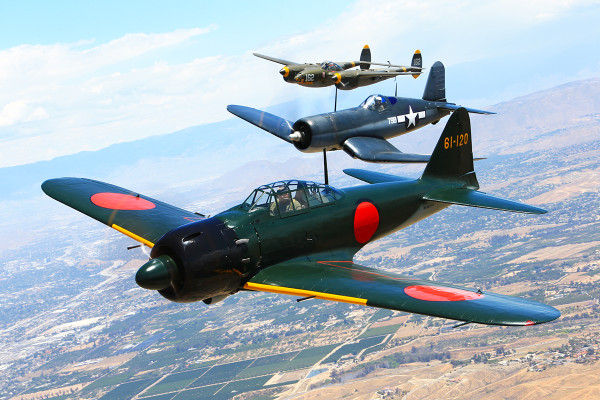
\includegraphics[width=140mm]{reisen.JPG}
    \end{center}
  \caption{零戦実機}
 \label{fig:reisen}
\end{figure}

\subsection{F6F ヘルキャット}
ヘルキャットとはアメリカの航空機会社であるグラマン社が製造した第二次大戦中アメリカ海軍の主力戦闘機である.良好な運動性能、急降下性能を有していたため日本の航空戦力を撃破するのに最も貢献した機体である.ズーム上昇は頑丈さゆえに急降下で速度を稼げるヘルキャットの方が零戦よりも優れている.さらに、急降下性能、武装、防弾性能、横転性能、旋回性能も、時速400km以下の速度域以外では零戦より優れていた.
ヘルキャットの図を図\ref{fig:F6F}に示す.

\begin{figure}[htbp]
  \begin{center}
    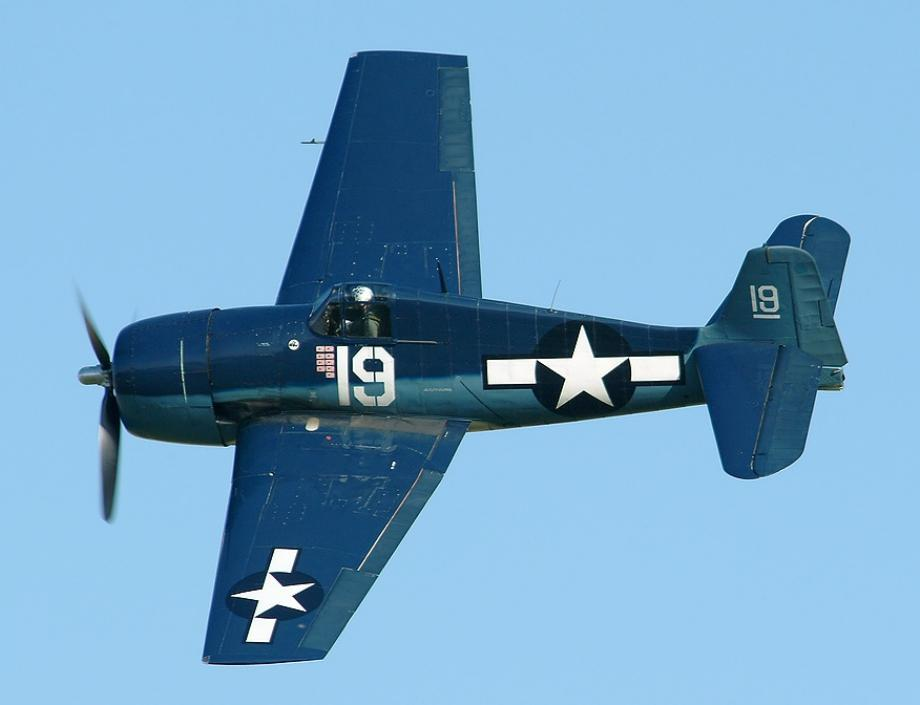
\includegraphics[width=140mm]{F6F.JPG}
    \end{center}
  \caption{ヘルキャット実機}
 \label{fig:F6F}
\end{figure}

\section{試作機の図面の製作方法}
図面を制作する際,まずインターネットで零戦とヘルキャットの図面を検索し図面を印刷する.その後図面の寸法を定規を用いて測り,(ストローの全長/図面の全長)*測りたい部分の長さの公式を用いて長さを算出した後CADを用いて図面を作成する.
算出の結果,零戦の主翼の全長は205.8mm,尾翼の全長は88.8mm,垂直尾翼の全高は30.4mmという結果になった.寸法入りの図面を図\ref{fig:mainwing},\ref{fig:tail}に示す.また零戦完成モデルの写真を図\ref{fig:sen}に示す.

\begin{figure}[htbp]
  \begin{center}
    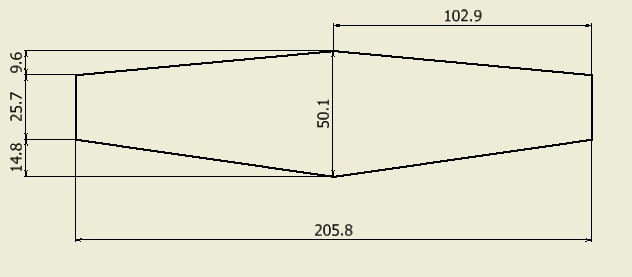
\includegraphics[width=140mm]{mainwing.JPG}
    \end{center}
  \caption{零戦主翼図面}
 \label{fig:mainwing}
\end{figure}

\begin{figure}[htbp]
  \begin{center}
    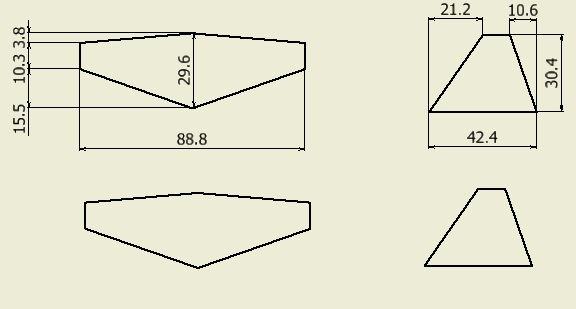
\includegraphics[width=140mm]{tail.JPG}
    \end{center}
  \caption{零戦図面}
 \label{fig:tail}
\end{figure}

\begin{figure}[htbp]
  \begin{center}
    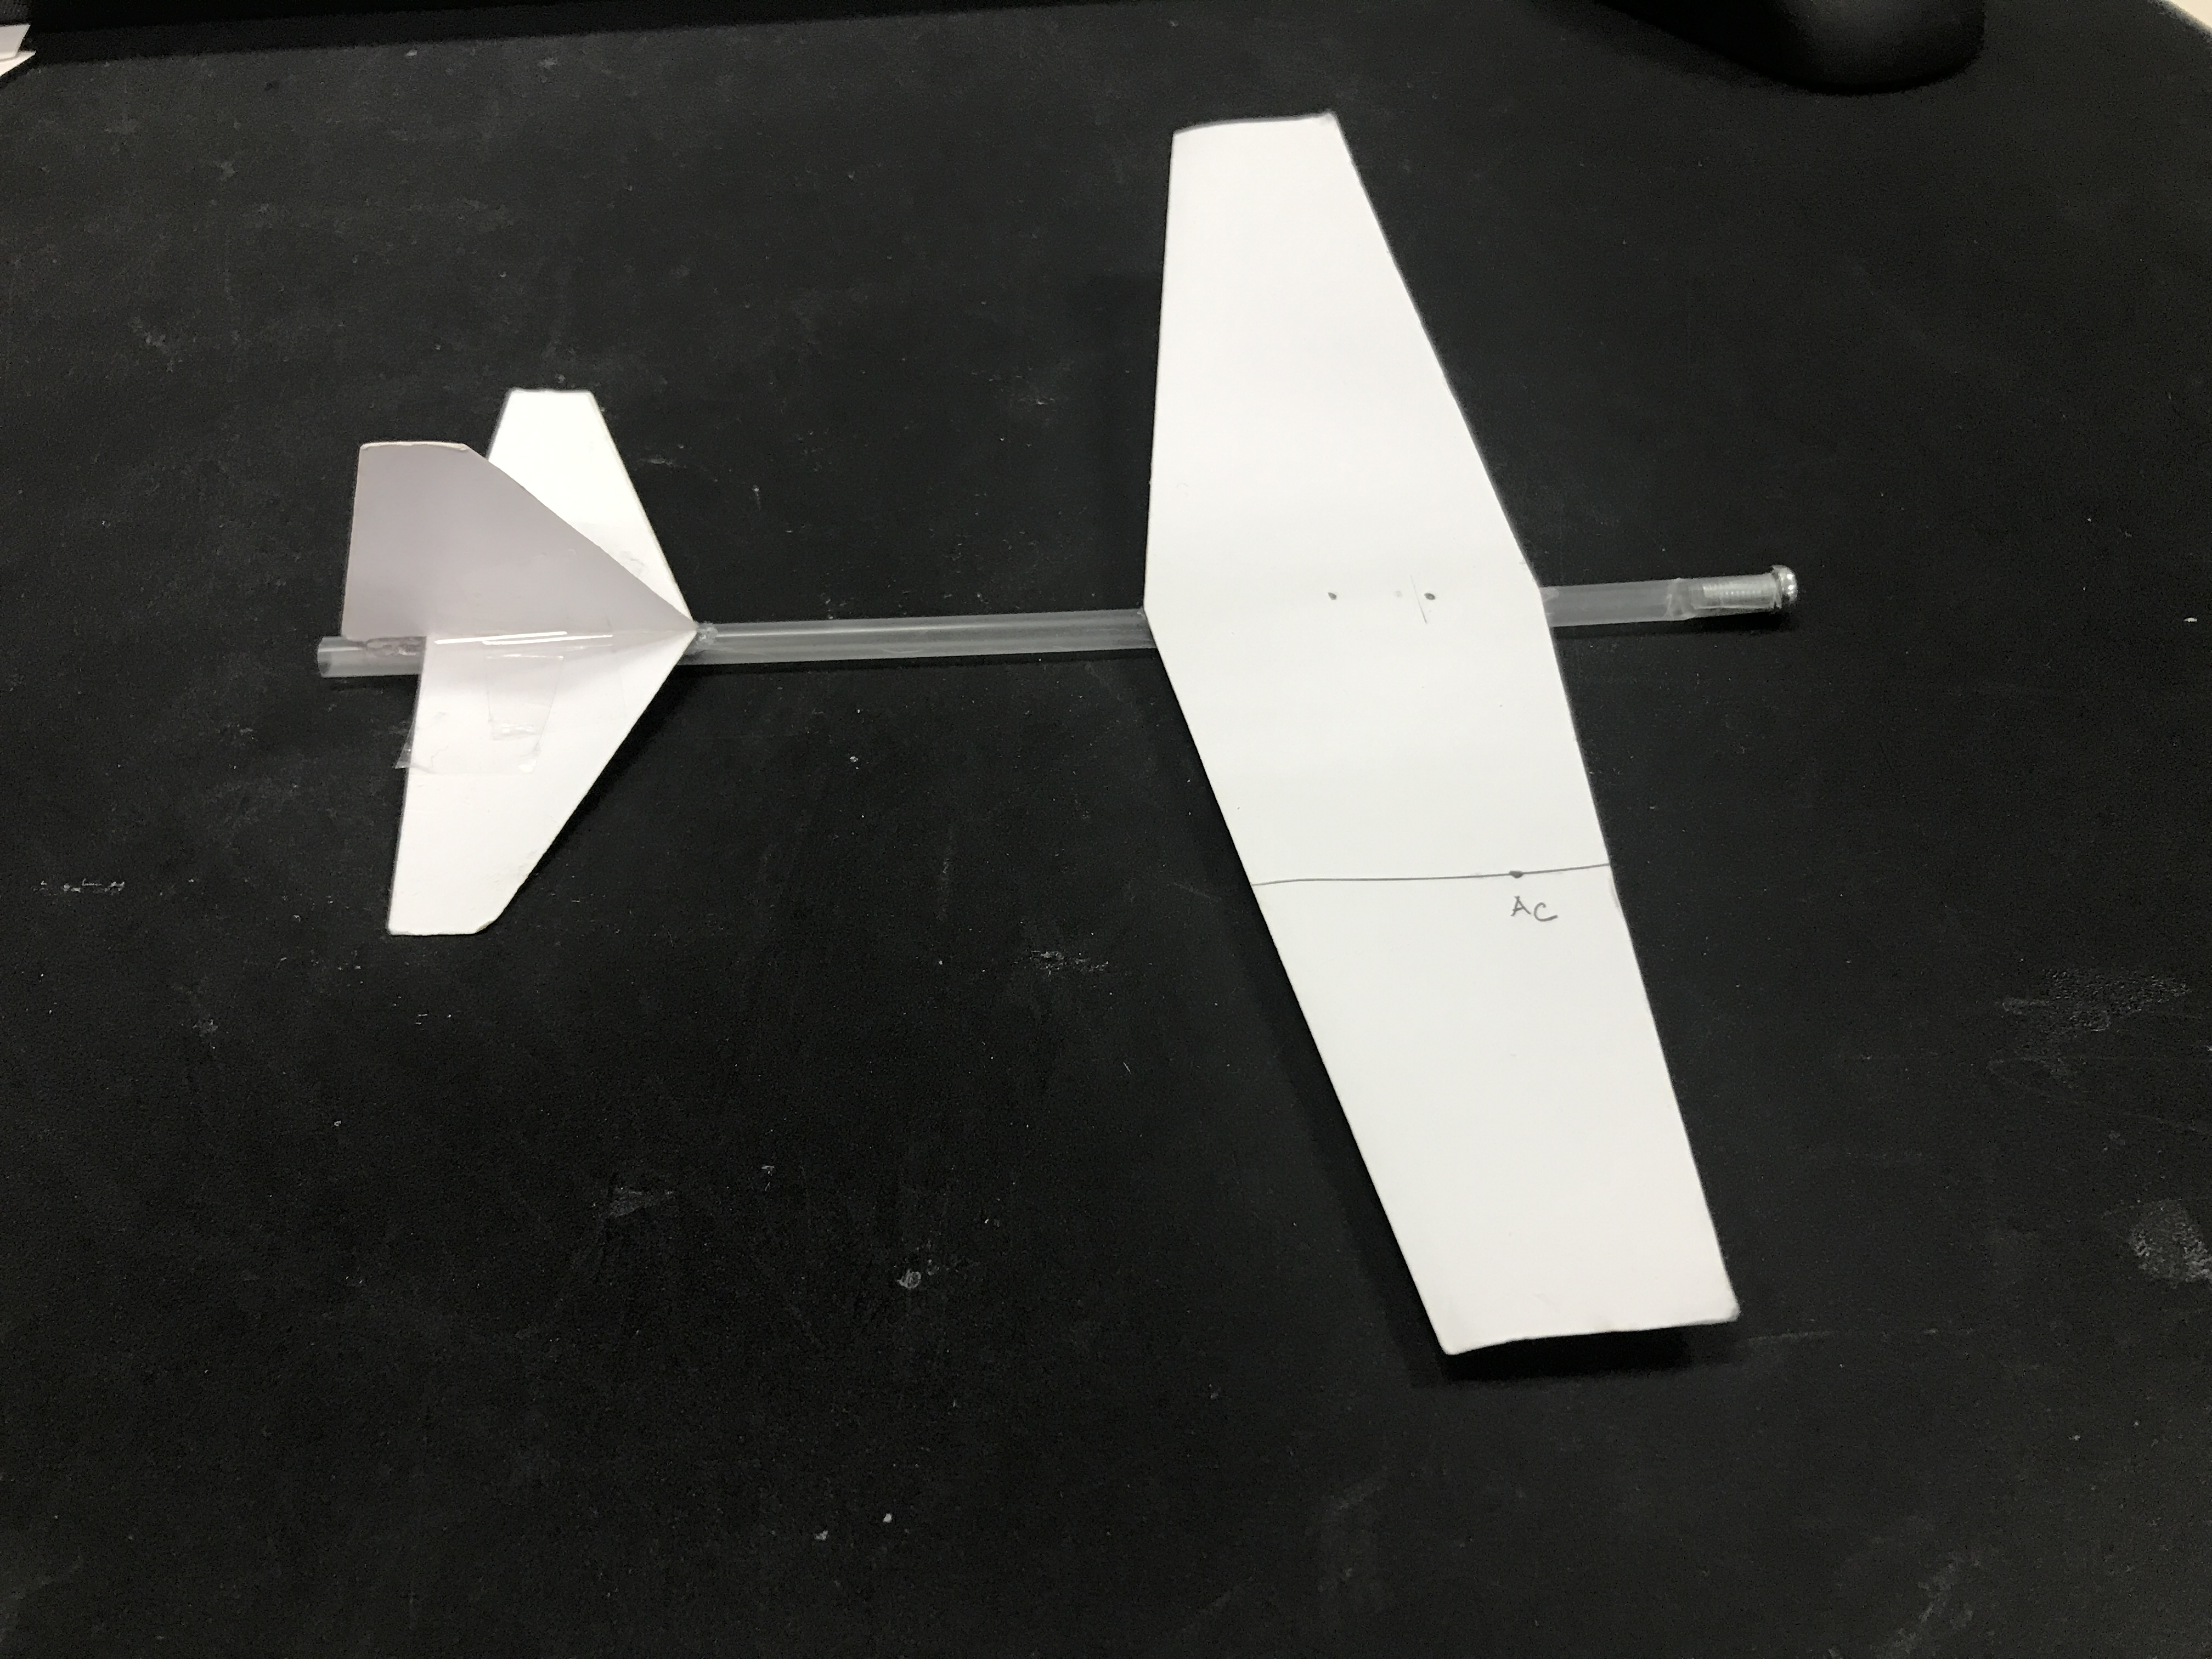
\includegraphics[width=140mm]{sen.JPG}
    \end{center}
  \caption{零戦}
 \label{fig:sen}
\end{figure}


次にヘルキャットの算出を行った結果,主翼の全長は242.4mm,尾翼の全長は108.2mm,垂直尾翼の全高は28.5mmという結果になった.寸法入り図面を図\ref{fig:guramanmainwing},\ref{fig:guramantail}に示す.またヘルキャット完成モデルの写真を図\ref{fig:man}に示す.

\begin{figure}[htbp]
  \begin{center}
    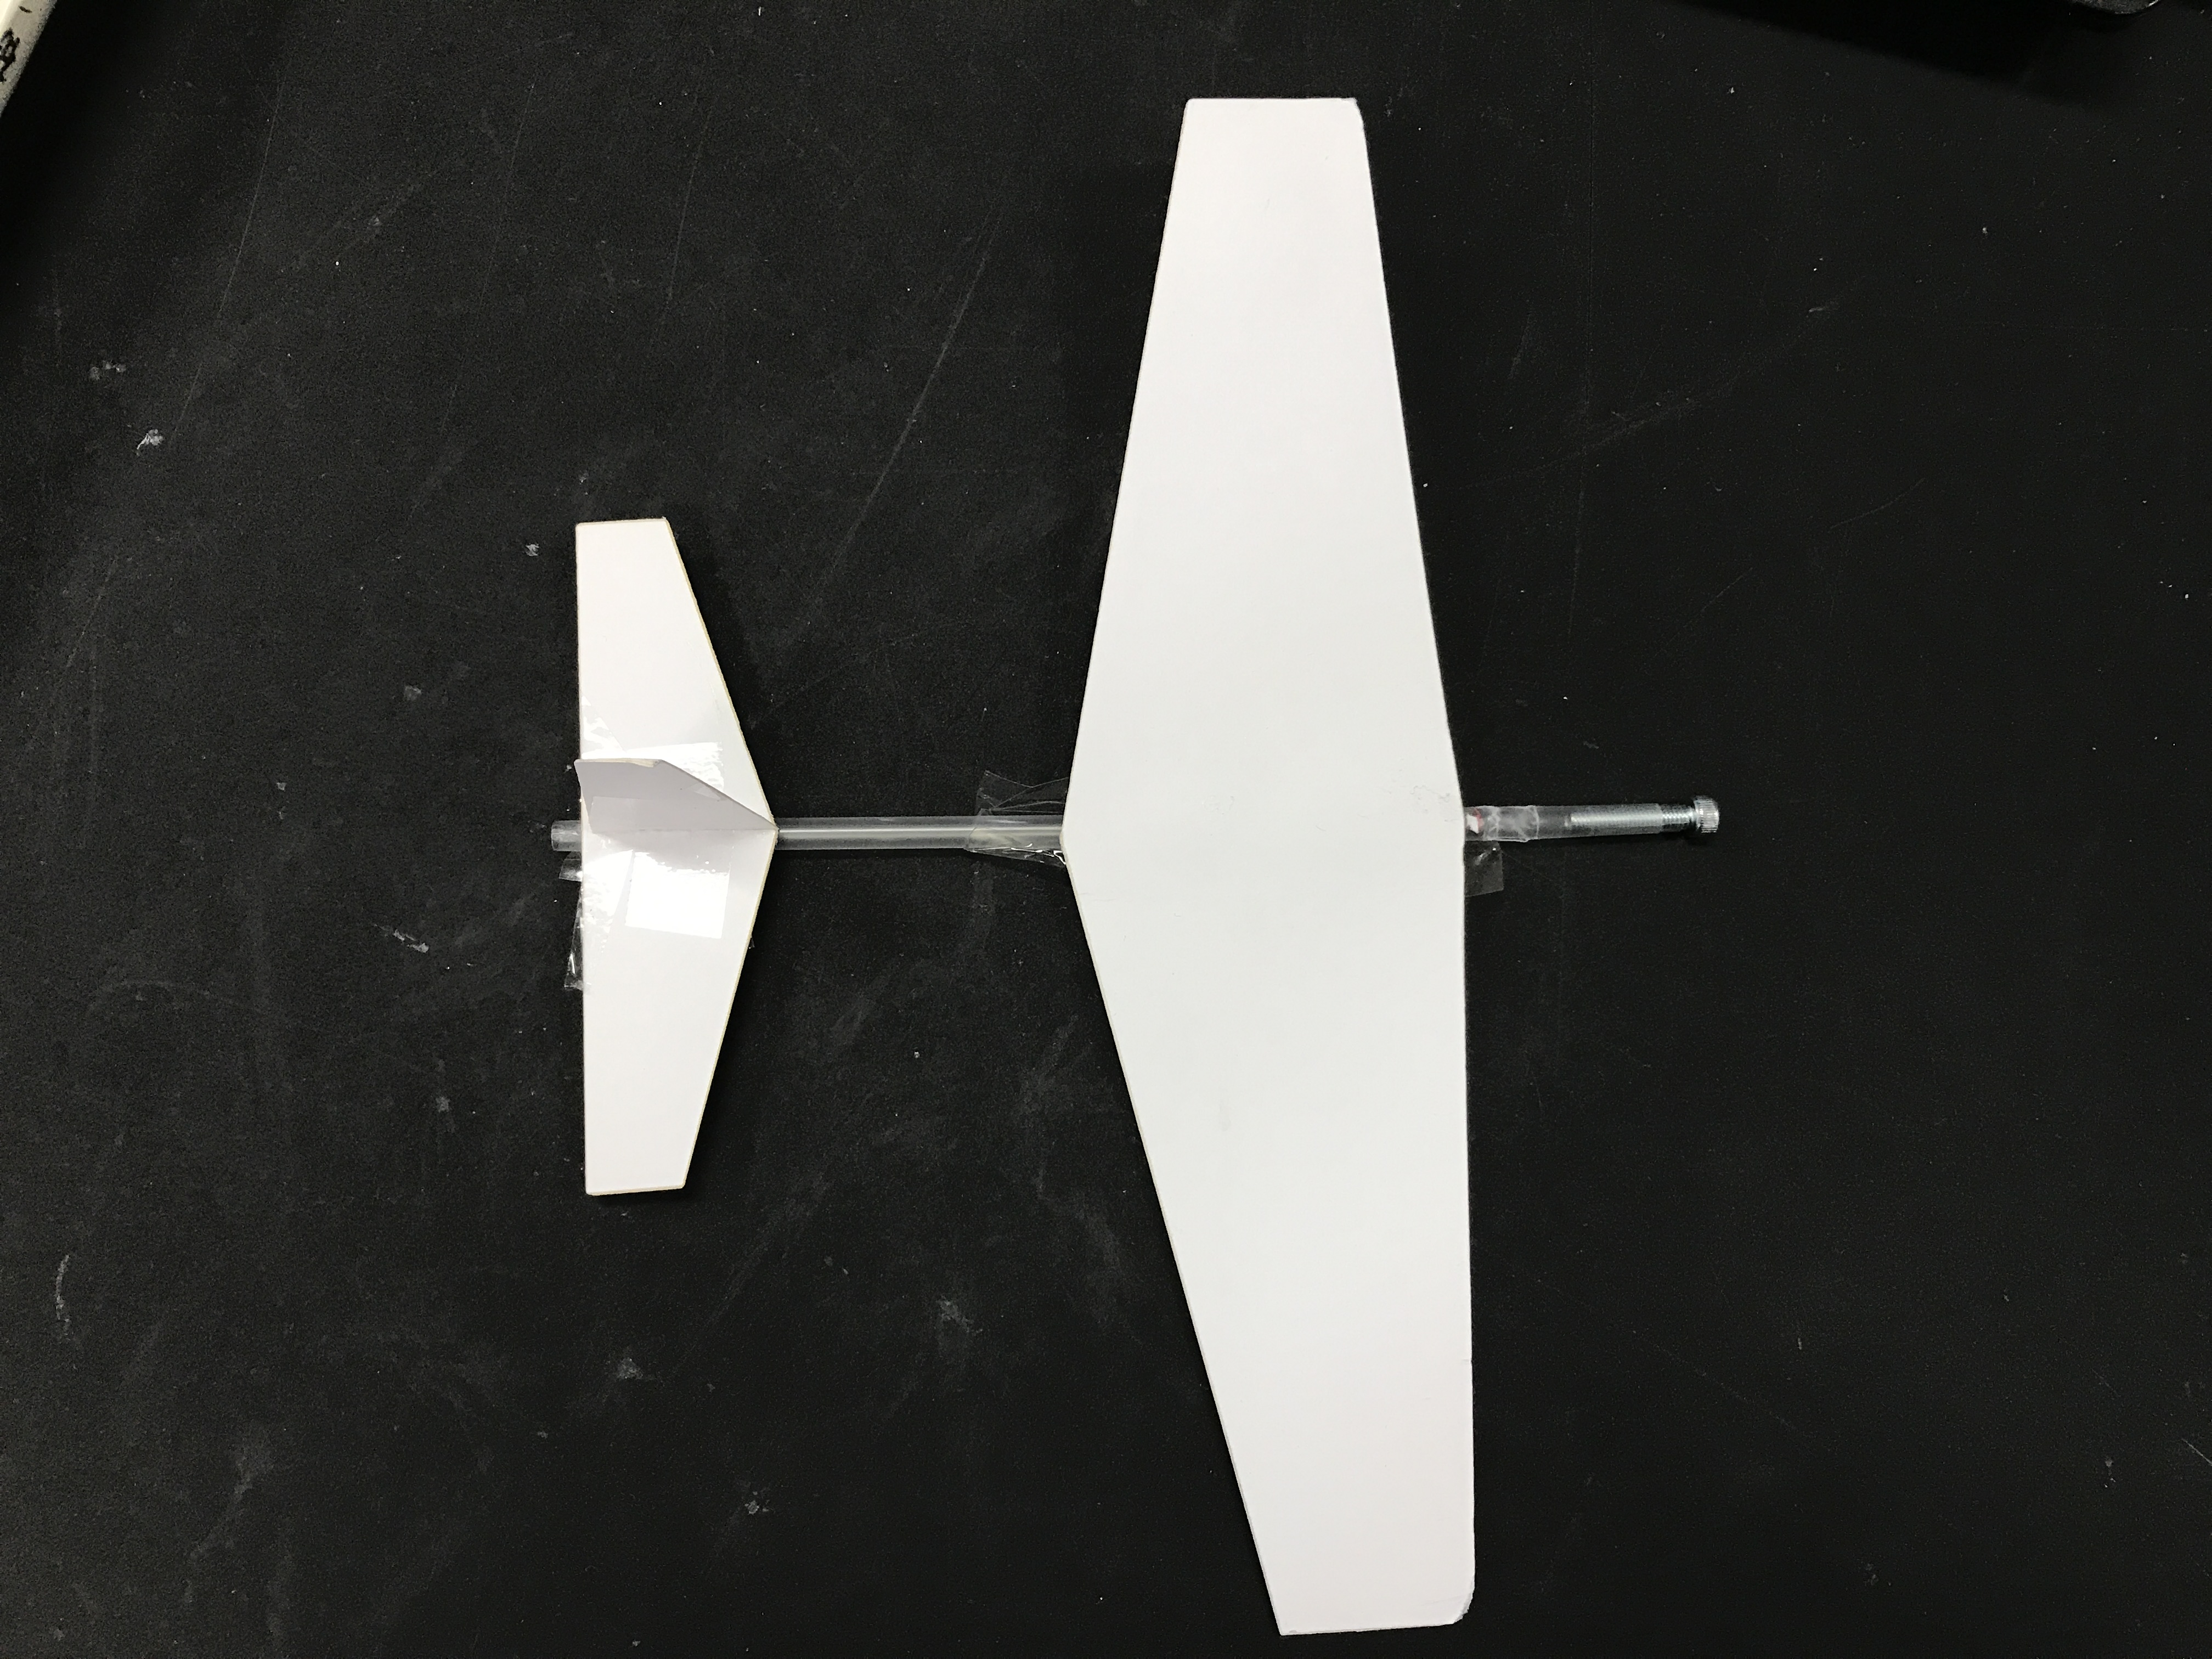
\includegraphics[width=140mm]{man.JPG}
    \end{center}
  \caption{ヘルキャット}
 \label{fig:man}
\end{figure}

\begin{figure}[htbp]
  \begin{center}
    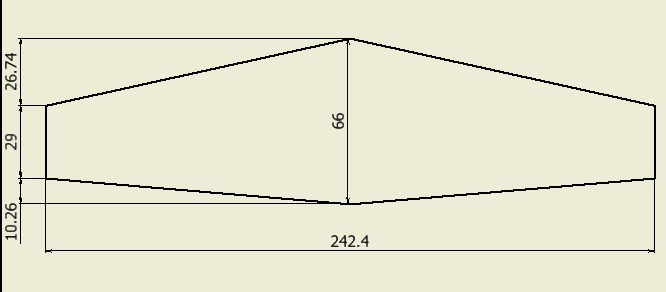
\includegraphics[width=140mm]{guramanmainwing.JPG}
    \end{center}
  \caption{ヘルキャット主翼図面}
 \label{fig:guramanmainwing}
\end{figure}

\begin{figure}[htbp]
  \begin{center}
    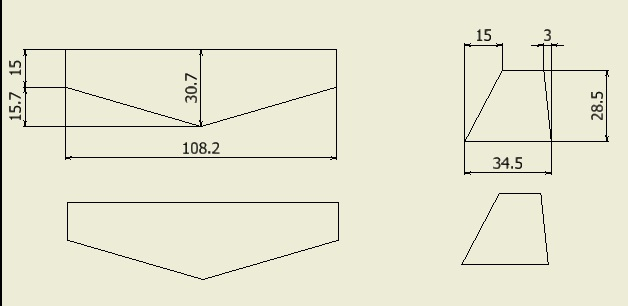
\includegraphics[width=140mm]{guramantail.JPG}
    \end{center}
  \caption{ヘルキャット図面}
 \label{fig:guramantail}
\end{figure}

図面から零戦よりもヘルキャットの方が翼が大きいことが分かる.またテーパ比は零戦が0.513,ヘルキャットが0.439,翼面積は零戦が7800,ヘルキャットが11514という結果になった.このことからテーパ比は零戦の方が大きいが翼面積はヘルキャットの方が大きいことが分かる.以上より零戦は機体の軽快性に優れていると考えヘルキャットは機体の安定性に優れていると考える.

\section{飛行機の縦の安定性}
飛行機が安定して真っすぐ飛ぶためには機体の重心位置がとても関係がある.もし重心位置を考えなかった場合,機体が宙返りしたり飛んだ瞬間頭から落ちる現象が発生する.したがって作図と計算を用いて重心位置の算出を行った.
\subsection{空力中心}
主翼はある一定の中心点を中心に揚力が発生するとみなすことが出来る.その点を空力中心と呼ぶ.空力中心を求めるためには計算でも求める事が可能だがテーパ翼では作図を用いて求める事が多い.したがって今回は作図を用いて求める方法を紹介したいと思う.
まず初めに主翼の片翼だけの図面を印刷する.その後下図\ref{fig:yoku}のように作図を行う.交点から約25割の位置が空力中心である.交点から垂直に線を伸ばし翼中央と交わった所がその翼の一番揚力が発生する位置である.
したがって今回作成した零戦の場合,空力中心位置が後ろから130mm,重心位置が後ろから121mmの位置にあるため機体が頭上げの動作を行う構造となっている.頭上げを行うと機体が宙返りしたりするため真っすぐ機体が飛ぶ確率が低い.そのため空力中心と重心位置を出来るだけ近づけた方が安定して機体が飛ぶ事が出来る.
\begin{figure}[htbp]
  \begin{center}
    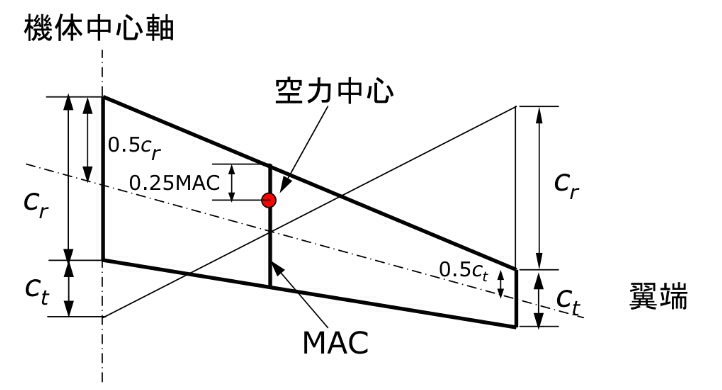
\includegraphics[width=140mm]{yoku.JPG}
    \end{center}
  \caption{空力中心の求め方}
 \label{fig:yoku}
\end{figure}
